\documentclass{article}
\usepackage[utf8]{inputenc}
\usepackage[spanish]{babel}
\usepackage{ifpdf}
\usepackage{hyperref}
\usepackage{subcaption}
\usepackage{graphicx}
\usepackage{textcomp}
\usepackage{caption}
\usepackage{mathtools}
\usepackage{enumerate}

%\usepackage[caption = false]{subfig}

\title{Operación y Mantenimiento Primario de Instrumentos, Equipos e Instalaciones Eléctricas y Electrónicas de la Aeronave}
\author{...}
\date{2015}
\ifpdf
\hypersetup{
    pdfauthor={...},
    pdftitle={Operación y Mantenimiento Primario de Instrumentos, Equipos e Instalaciones Eléctricas y Electrónicas de la Aeronave
},
}
\fi

% Para cambiar los nombres por defecto:
% Babel traducía table como cuadro. Yo lo cambio para tabla:
\addto\indexspanish{%
  \renewcommand{\indexname}%
    {Programa de la materia}%
}

\begin{document}
\maketitle
\pagebreak
\tableofcontents
\pagebreak
		

\subsection{Altímetros}
\subsubsection*{Generalidades}
El altímetro es un instrumento que permite medir altura basado en la variación vertical de la presión de la atmósfera. La calibración de su escala está hecha bajo condiciones de atmósfera Standard y en consecuencia, sólo indicará valores reales cuando se den estas condiciones.
Siendo la atmósfera un medio esencialmente variable, fue necesario definir la llamada ``Atmósfera Standard'', para contar con una referencia universal de calibración de los instrumentos. Además fue necesario establecer un procedimiento de ajuste para adecuarse a las circunstancias locales en cada momento.

``Atmósfera Standard'' es un estado atmosférico que cumple los siguientes requisitos:

\begin{itemize}
\item A nivel medio del mar (MSL), la presión barométrica es 760 mm. de columna de mercurio ($29,92"$ de Hg, ó $1013,2$ hectopascales).
\item La temperatura en el mismo punto es de 15°C (59°F).
\item La aceleración de gravedad es de 9,806 m/seg. al cuadrado y se asume que bajo 65.000¹ no hay cambios significativos. Se considera aire seco.
\item El gradiente de temperatura para altitudes entre 0 y 35.332 pies (troposfera), es lineal, descendente e igual a 0,65°C cada 100 mts. de incremento de altitud. (1°F/$280'$).
A partir de 35.332' (límite de estratosfera) y hasta 104.987' la temperatura es constante e igual a -55°C (-67°F).
\end{itemize}
Los altímetros considerados, llamados de tipo Kollsman, están calibrados para esta atmósfera Standard y específicamente para la curva de presiones de la zona inferior o troposfera.
En esta zona, la presión se rige por la ecuación:

$$P = 29,92 \times(\frac{288 - 0,0019812Z}{288})^{5,26}$$


En que $P$ es la presión en pulgadas de Hg a la altitud $Z$ (pies). Esta altitud $Z$, se denomina \textbf{Altitud de Presión} y es la Altitud en Atmósfera Standard donde existe el valor de presión considerado.
La variación de presión a baja altitud es aproximadamente de $1"$ cada $1.000'$ y descendente con el aumento de altitud.
La variación de la temperatura Standard es aproximadamente de $2^{\circ}\mathrm{C}$ cada $1.000'$ (exactamente 1,9812°C), descendente y de valor constante con la altitud hasta alcanzar $35.332'$.
Algunos puntos singulares de esta atmósfera Standard son:


$$17.965' \text{de~altitud} = \text{Presión atmosférica media~ de la Standard}$$

$$35.332' \text{de~ altitud}  = \text{Comienza la estratosfera}$$
\begin{equation}
7.571' \text{de~ altitud}  = \text{Altitud Standard de la Isoterma 0}
\end{equation}
\subsubsection*{Usos del altímetro}
\begin{center}
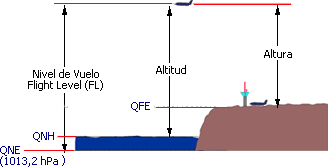
\includegraphics[scale=0.75]{figuras/alturas.png}
	\captionof{figure}{\emph{Altura, altitud y nivel de vuelo}.}
\label{fig:alturas}
\end{center}

Aún habiendo sido la intención original del desarrollo del altímetro la función de medir altitudes reales, la evolución práctica de su uso ha conducido a otras funciones, que si bien usan el mismo concepto, se diferencian en su objetivo.

Los usos específicos actuales son:
\paragraph{Separación entre aeronaves.}
Si se usa una referencia común de calibración de los altímetros, al asignar niveles de vuelo distintos a diferentes aeronaves medidos con este instrumento, se asegura, sin otra corrección, su separación vertical.
Para este fin se ha adoptado convencionalmente el valor de referencia 29,92" (QNE), correspondiente al nivel 0 de atmósfera Standard, para el ajuste de altímetro de todos los aviones volando sobre o fuera de las zonas de
aproximación (en las que se ajusta a QNH). De este modo todos los aviones vuelan superficies de presión de referencia común, a las que se llama Niveles de Vuelo y se designan en cientos de pies. Ej.:10.000' se expresan como FL 100.
Corresponde este concepto exactamente al de Altitud de Presión definido con la Atmósfera Standard.
\paragraph{Indicación convergente a la elevación de la pista.}
Usando un ajuste de altímetro igual al QNH informado por la torre de control de la pista en que se va a aterrizar, se asegura, sin otra corrección, una indicación igual a la elevación de la pista cuando se toma contacto con ella.
Esta condición permite referencias comunes de altitud a los aviones en circuito de tránsito de aeródromo o en fase de aproximación y garantiza además vuelo seguro en áreas definidas, a condición de respetar las holguras establecidas para el franqueamiento de obstáculos.
Se ha usado el término indicación convergente, por cuanto sólo al nivel de la pista se obtiene del altímetro una indicación verdadera, salvo condiciones de atmósfera Standard.
\paragraph{Información barométrica.}
Calibrado en QNE (29,92"), el altímetro da información de presión barométrica, expresada en pies de altitud según atmósfera Standard, necesaria para efectuar correcciones de velocímetro, de altímetro y para cálculo de altitud de densidad.
\paragraph{Determinación de la Altitud Verdadera.}
Al aplicar a las indicaciones del altímetro las correcciones de presión, mediante ajuste a QNH, y de temperatura, por cálculo mediante el computador Dalton o sus equivalentes, se obtiene la altitud verdadera de la aeronave sobre el nivel medio del mar.
La afirmación anterior tiene una excepción y es el caso en que el gradiente térmico vertical de la atmósfera no es lineal. La linealidad es condición básica que sustenta todos los cálculos de altimetría. Afortunadamente es, dentro de una razonable aproximación, la condición más habitual de la atmósfera.


\subsubsection*{Principios de funcionamiento}

\begin{figure}
\begin{center}
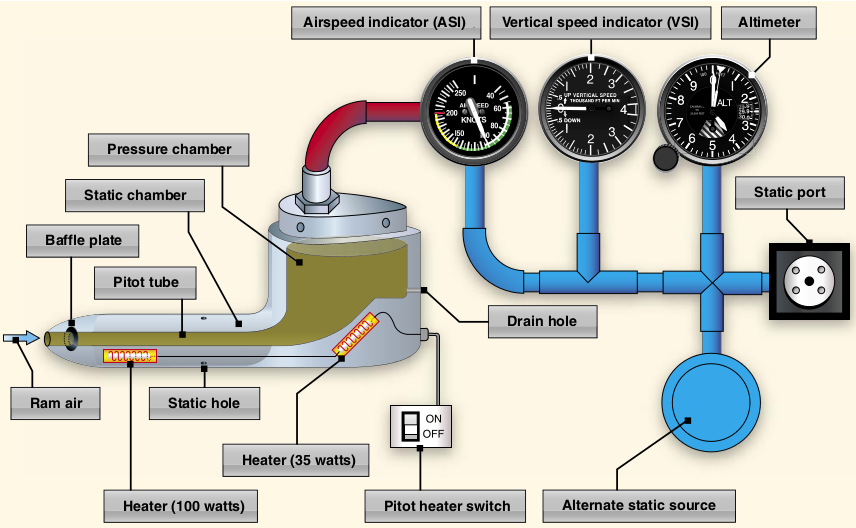
\includegraphics[scale=0.45]{figuras/pitostatico.png}
\caption{Sistema Pitot-Estático}
\label{pstati}
\end{center}
\end{figure}


El altímetro es un barómetro de tipo aneroide conectado al conducto de Presión Estática del Sistema Estático Pitot, cuyas indicaciones de altitud aparecen sobre una escala graduada en PIES, unidad adoptada como Standard por la OACI. La escala en referencia, está calibrada bajo condiciones Standard de atmósfera, pero dispone de un mecanismo de corrección que permite ajustarla según las variaciones de la presión barométrica. El ajuste se efectúa en otra escala que se muestra a través de la llamada ventanilla Kollsman.

\begin{figure}
\begin{center}
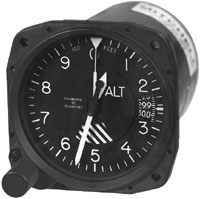
\includegraphics[scale=0.75]{figuras/altimetro-1.jpg}
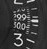
\includegraphics[scale = 0.99]{figuras/altimetro-1b.jpg}
\caption{Ejemplo de un altímetro y un acercamiento a la ventanilla Kollsman }
\label{some example}
\end{center}
\end{figure}

QNH es el valor de la presión atmosférica a nivel medio del mar (MSL) o Nivel Cero, en una atmósfera de gradiente térmico Standard. Al ajustar el altímetro a este valor en la ventanilla Kollsman, se debe lograr una indicación Cero de las agujas sobre su carátula cuando el altímetro se encuentre en la posición Nivel Medio del Mar. De esta manera se logra que, ante un cambio de la presión atmosférica, el altímetro pueda ser ajustado para que vuelva a medir altura con respecto a ese mismo nivel. A esta indicación, una vez efectuado el ajuste de QNH, se le denomina Altitud Indicada.

Al contar el altímetro con este dispositivo de ajuste de la presión de referencia, se abre la posibilidad de medir alturas sobre cualquier nivel de presión que se elija. Esta segunda forma de ajuste permite que, si este nivel es el existente a la elevación de la pista de un aeródromo, (QFE), el altímetro, ajustado a esa referencia medirá altura sobre dicha elevación, e indicará CERO cuando el 
avión esté posado sobre la pista.

El rango de ajuste de presiones del altímetro tiene límites, de modo que lo anterior no es posible para aeródromos de gran elevación. Este rango, que se muestra en los extremos de la escala de la ventanilla Kollsman, está comprendido entre 28,1 y 31,0 pulgadas de Hg.

Este último tipo de ajuste no es válido para vuelo por instrumentos y tampoco es comúnmente usado. Sólo tiene sentido en condiciones especiales de vuelo como es el caso de la acrobacia o de los planeadores.

Una tercera forma de calibración del altímetro resulta de ajustarlo a la Presión Standard de 29,92" de Hg. (QNE). En este caso se está usando el altímetro en la misma forma que si no tuviera mecanismo de ajuste de presiones. Su curva de calibración es ahora la que corresponde a la Atmósfera Standard y en consecuencia va a medir altitud sobre una superficie de referencia cuya presión es 29,92" de Hg. A esta altitud se la denomina Altitud de Presión teniendo como sinónimo el término Nivel de Vuelo, usado por el ATC para fines de control de tráfico.

\subsubsection*{Construcción}
El mecanismo del altímetro está constituido por una cápsula aneroide hermética, contenida en una caja sellada, que se conecta a la línea de presión estática del sistema Estático-Pitot. Esta presión, al actuar sobre la cápsula, produce en ella un mayor o menor aplastamiento según sea su magnitud, efecto que se emplea para accionar el sistema indicador.
Normalmente, para hacer más sensible al sistema, se acoplan tres cápsulas en serie.


\begin{center}
	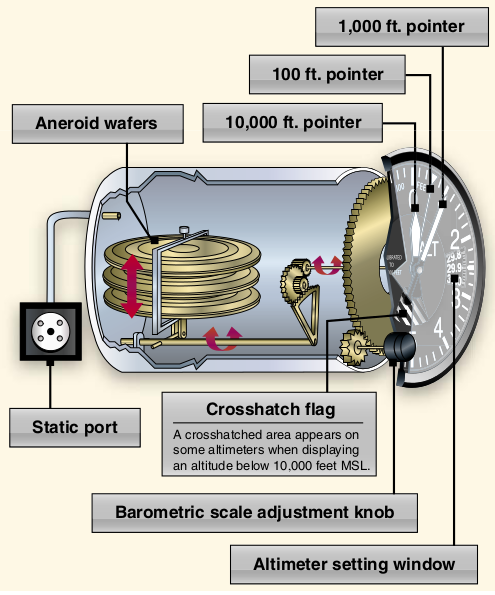
\includegraphics[scale=0.5]{figuras/anemometro.png}
	\captionof{figure}{\emph{Altímetro}.}
\label{fig:alt-1}
\end{center}
Las cápsulas se fijan por un extremo, a la caja sellada del instrumento, a través de un mecanismo de calibración, mientras que por el otro extremo se unen a las agujas indicadoras a través de un mecanismo de relojería que convierte los desplazamientos de las cápsulas en rotación del eje de las agujas. Todo el conjunto está estabilizado térmicamente mediante bimetales correctores, que lo hacen prácticamente insensible a los cambios de temperatura. Dispone además de ajustes de ganancia que permiten calibrar la escala a la curva teórica de la Atmósfera Standard.

El conjunto aneroide-mecanismo de relojería, está montado fijo a un disco, que al girar accionado por la perilla ya mencionada, permite el ajuste de presiones o ajuste de QNH.

En el extremo del eje central del altímetro y fijo a la carátula del instrumento, existe un mecanismo reductor de doble relación 1/10 que es el que acciona las 3 agujas indicadoras.


\subsubsection*{Lectura}
La carátula del altímetro muestra una escala circular marcada de 0 a 9 y con 5 líneas entre cada número que corresponden a divisiones de 20 pies.

Sobre ella se mueve una aguja primaria (la mayor en tamaño), para la cual cada número representa cien pies, o sea, 1.000'/vuelta.
A través del mecanismo reductor antes mencionado, se acciona una segunda aguja (de menor tamaño) cuyo movimiento indica 1000 pies por número, o sea, 10.000'/vuelta.

En vista de que a 10.000' el altímetro presentaría el mismo aspecto que a 0', el mismo mecanismo reductor acciona una tercera aguja que permite distinguir en qué tramo de la indicación se está.


\subsubsection*{Ajustes}
\paragraph{Efecto de presión.}
El procedimiento de ajuste altimétrico establece que siempre debe usarse el QNH informado por la torre o Centro de Control, cuando se vuela bajo el Nivel de Transición o hasta la Altitud de Transición, aún cuando el gradiente térmico no sea Standard. Esto porque, como ya se dijo, este procedimiento da indicación exacta a la elevación de la pista del aeródromo que da la información, estando los errores de indicación en altura, derivados de este tipo de ajuste, contemplados en el diseño del canal de aproximación.

Altitud de Transición es una Altitud Indicada, con QNH, que garantiza franqueamiento de obstáculos en un radio alrededor de un aeródromo o en un sector de un Área Terminal. Es un valor fijo que se establece para cada lugar. Durante un ascenso debe mantenerse referencia QNH hasta la Altitud de Transición publicada y debe ajustarse a QNE (29,92") desde esa altitud hacia arriba.

Nivel de Transición es el nivel mínimo utilizable, con QNE, que garantiza franqueamiento de obstáculos en las condiciones descritas. Es un valor variable según las condiciones atmosféricas, que es establecido por el Centro de control para cada lugar y cada momento. Durante un descenso, debe mantenerse referencia QNE hasta el Nivel de Transición informado por el Centro y debe ajustarse a QNH desde ese nivel hacia abajo.

Las Torres de Control de los aeródromos principales, obtienen el valor de su presión atmosférica por lectura de un barómetro patrón, de calibración muy perfecta, al cual se ha aplicado una corrección para reducir esta lectura a
su valor a nivel del mar o QNH. Esta reducción se hace según los valores que corresponden a atmósfera Standard y por lo tanto, la corrección para una determinada Torre, siempre es la misma. Esto trae dos consecuencias, la primera es que se logra indicación exacta a la elevación de la pista y la segunda es que el QNH resulta diferente para aeródromos de distinta elevación, aunque estén muy cercanos.

El primer ajuste de presión del altímetro debe hacerse en la losa antes del vuelo. El procedimiento establece:
\begin{itemize}
\item Ajustar la ventanilla Kollsman al QNH indicado por la torre.
\item Comparar la indicación del altímetro con la elevación del aeródromo.
\item Aceptar, para vuelo IFR, un Error máximo de 75'.
\end{itemize}
Es necesario considerar que cuando se ingresa a una zona de mayor presión que la que ha servido de referencia para ajuste del altímetro, la indicación de éste sería menor si se pudiera mantener la altitud verdadera, pero como el piloto mantiene la altitud indicada, resulta volando a mayor altitud que la que el altímetro indica. Naturalmente lo contrario sucede al ingresar a una zona de menor presión.

\paragraph{Efecto de Temperatura.}

Una vez efectuado el ajuste de presión recién descrito, el altímetro queda calibrado para dar indicación correcta, cuando a la altitud indicada, el valor de la temperatura es el que corresponde a esa altitud en la atmósfera Standard. Si la temperatura actual es diferente de la Standard, habrá una rotación en las curvas de presión y la indicación del altímetro no será correcta.

En los tres primeros usos definidos para el altímetro, no se requiere ninguna corrección por efecto de temperatura. Para el cuarto, determinación de la altitud verdadera, es necesaria esta corrección.

El computador Dalton facilita la aplicación de esta corrección, que responde a la siguiente ecuación:

$$ \text{Altitud verdadera} = \frac{\text{Temperatura actual en Kelvin}}{\text{Temperatura Std. del FL en Kelvin}}\times\text{altitud indicada}$$

De manera semejante al caso de la presión, si se ingresa a una zona de mayor temperatura, con referencia QNH constante, se está volando más alto que lo indicado.

La razón de esta diferencia, está en que la expansión o contracción vertical de la atmósfera causada por los cambios de temperatura, produce un desplazamiento vertical de los niveles de presión a los que responde el altímetro.



\subsubsection*{Errores del altímetro}
\begin{enumerate}[a.]
\item Error de escala. Se debe a la calibración de sólo 1000' de escala (una vuelta de la aguja primaria), de acuerdo a un tramo bajo de la curva de presión de la atmósfera Standard y a la extrapolación de este tramo a todo el rango de indicación del altímetro en el que se encuentran gradientes de presión progresivamente diferentes con la altura. De hecho, no es posible utilizar repetitivamente una misma escala, cuando la variación del fenómeno medido no es lineal. Por esto, la tolerancia a este error es variable y así un error de + -200' a FL400 puede ser perfectamente aceptable.
\item Error mecánico. Se debe a desalineamiento del mecanismo que relaciona la indicación de las agujas con la escala de ajuste. Es el que se verifica en la inspección prevuelo y que no debe ser superior a 75 pies.
\item Error de fricción. Es el causado por roce entre las piezas móviles del mecanismo y que se anula por vibración.
\item Error de Histéresis. Es un error causado por deformación diferida del material que se manifiesta después de vuelos largos a grandes alturas. Es como un acostumbramiento de la cápsula aneroide a su nueva posición que
retarda el cambio de la indicación.
\end{enumerate}

\subsubsection*{Tipos de altura}

Las siguientes definiciones resumen los conceptos de altura hasta aquí utilizados:
\begin{description}
\item[Altura Absoluta:] Separación vertical entre el avión y la superficie o terreno sobre el cual está volando.
\item[Altitud Indicada:] Es la lectura del altímetro ajustado a la presión barométrica del momento (QNH)
\item[Altitud Calibrada:] Es la altitud indicada corregida por error de escala según cartilla.
\item[Altitud Verdadera:] Es la separación vertical del avión con respecto al nivel del mar.
\item[Altitud de Presión o Nivel de Vuelo:] Es la lectura del altímetro ajustado a 29,92" de Hg. Corresponde a la separación vertical del avión con respecto a una superficie de presión de 29,92" de Hg., denominada plano de referencia
Standard.
\item[Altitud de Densidad:] Es la altitud de presión corregida por temperatura. Corresponde a la altitud en atmósfera Standard a la cual existe el valor de densidad observado.
\end{description}



\subsubsection*{Mantenimiento del instrumento}
Para determinar la condición del instrumento, ajustar la escála barométrica según el dato de presión brindado por una estación meteorológica de confianza local. El altimetro debe indicar la altura del lugar sobre el nivel del mar. Si la altura indicada tiene un error mayor a los 75 pies, el instrumento requiere ser recalibrado.




\subsection{Variómetro}
\subsubsection*{Introducción}
Otro de los instrumentos básicos derivados del Sistema estático pitot, es el Variómetro. Basado en la variación vertical de la presión atmosférica y no siendo ésta de característica lineal, requiere de un diseño muy ingenioso para compensar diferencias debidas a su uso en distintas altitudes y lograr una razonable constancia en el régimen indicado de ascenso o descenso.

\subsubsection*{Generalidades}
Si bien el Variómetro no es un instrumento imprescindible, como se entienden ser el Altímetro y el Velocímetro, forma con ellos un grupo que es esencial para el control longitudinal del vuelo de precisión. Actúa en general como un instrumento de apoyo, pero también como un instrumento primario cuando el objetivo de la maniobra es lograr un ascenso o descenso a razón constante.

Es un medidor de velocidad vertical que colabora significativamente en la precisión del vuelo, especialmente en condiciones IMC.
En razón de su principio de funcionamiento, su lectura debe efectuarse sólo bajo condición de indicación estable, la que se logra típicamente 6 a 9 segundos después de establecer una actitud constante.

\subsubsection*{USOS DEL VARIOMETRO}
En el vuelo visual, se usa como instrumento de apoyo para obtener control longitudinal y en la medida que se avanza en experiencia a través de su uso, para conseguir suavidad y precisión en la ejecución de toda maniobra.

En vuelo por instrumentos, tiene la función indicada para el vuelo visual y además, como ya se mencionó antes, puede tomar el carácter de instrumento primario de control longitudinal en maniobras como la aproximación ILS, en la cual la razón de descenso es uno de los condicionantes básicos para la buena ejecución de la maniobra.

La forma de uso de este instrumento está subordinada siempre a actuar mediante correcciones longitudinales de actitud y no a intentar la interpretación directa de la indicación del instrumento. Este último procedimiento llevaría, en vista de su retardo característico de indicación, a una serie no convergente de correcciones exageradas, en cambio, la corrección por actitud ya sea visual o instrumental permite una convergencia rápida a la condición de lectura estable necesaria para su uso.

No es el variómetro un instrumento cómodo para mantener un vuelo nivelado. Para ese fin sólo pueden interpretarse sus tendencias de indicación que son muchas y continuas debido a su gran sensibilidad. Sin embargo muestra claramente los errores importantes de control longitudinal permitiendo al piloto reaccionar oportunamente.

\subsubsection*{Principio de funcionamiento}
\begin{center}
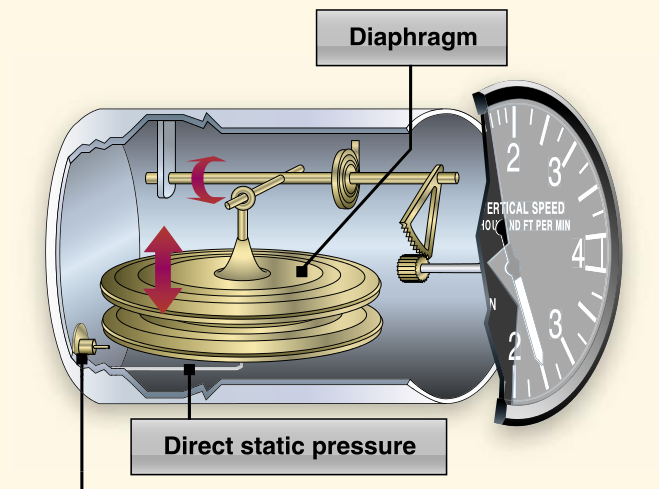
\includegraphics[scale=0.5]{figuras/vsi.png}
	\captionof{figure}{\emph{Variómetro}.}
\label{fig:alturas}
\end{center}
La presión estática captada en el sistema estático-pitot es función fundamentalmente de la altitud y además de otros parámetros como la temperatura. Estos determinan un gradiente vertical de presión en la atmósfera que sin ser lineal, permite ser la referencia de funcionamiento para este instrumento. En efecto, si se mide la variación de presión representativa de altitud y el tiempo en que esta variación se produce, se puede determinar la velocidad de desplazamiento vertical que es el objetivo del instrumento. El variómetro sólo mide el régimen de variación de la presión atmosférica y no es afectado por la temperatura del aire.

El método utilizado para este fin, producto de un notable ingenio de sus creadores, se basa en captar una muestra de presión estática y guardarla semi confinada en la caja del instrumento mediante un orificio calibrado permitiendo así, que si varía la presión estática exterior, la diferencia de presiones producida no se anule de inmediato sino con un retardo de algunos segundos. Es aquí donde se introduce la variable tiempo que permite calcular velocidad.

Dentro de esta caja se ubica una cápsula de tipo aneroide de características muy sensibles cuyo interior se conecta directamente a la presión estática externa.

Al ascender o descender la aeronave, la presión interior de la cápsula varía en forma casi instantánea mientras que la presión de la caja del instrumento aplicada a la superficie exterior de la cápsula, inicia una variación lenta que demora entre 6 y 9 segundos en anularse o en llegar a un valor de diferencia constante entre las dos presiones. Este valor es medido por la deformación elástica de la cápsula, la que a través de un mecanismo de relojería mueve una aguja sobre la carátula del instrumento, la que se calibra en pies por minuto de velocidad vertical.

La deformación de la cápsula se estabiliza cuando el flujo que permite el orificio calibrado determina un cambio de presión en la caja del instrumento de igual magnitud que el cambio de la presión atmosférica exterior causado por la variación de altitud. Aparece así una lectura instrumental que corresponde a la velocidad vertical de la aeronave. Una variación nula de presión se interpreta como vuelo nivelado y produce una indicación cero en el instrumento que se muestra con la aguja en posición horizontal izquierda.

Se tiene así que el ascenso de la aeronave produce un aplastamiento de la cápsula por la presión retenida actuando contra la presión interior decreciente y lo contrario durante un descenso. Las mayores deformaciones, esto es, las deflexiones máximas de la aguja se obtienen con diferencias de presión tan bajas como 0,05 pulgadas de mercurio lo que junto con mostrar la enorme sensibilidad del instrumento, advierte del peligro de aplicar presiones a las tomas estáticas, como por ejemplo soplar en ellas, lo que puede descalibrar o destruir el instrumento.

Pero los valores de las diferencias de presión actuantes no son constantes con la altura debido al gradiente no lineal antes mencionado. Esto llevaría a pensar que se obtendrán diferentes indicaciones a distintas altitudes para una misma velocidad vertical. Sin embargo, el diseño del instrumento permite reducir significativamente este efecto mediante el adecuado uso de un par de conceptos físicos que se relacionan con las diferencias de presión generadas por los escurrimientos de fluidos a través de tubos capilares y a través de orificios.

No es este artículo el lugar adecuado para desarrollar los fundamentos del uso de estos conceptos, pero debe entenderse que éste permite compensar en gran medida la no linealidad del gradiente vertical de presión de la atmósfera, al menos en el rango de uso del instrumento.

\subsubsection*{CONSTRUCCION DEL INSTRUMENTO}
Los elementos componentes del variómetro son: una caja hermética, una cápsula elástica de gran sensibilidad, una unidad de retardo, un mecanismo de relojería y una carátula de presentación.

La cápsula, unida por un extremo a la estructura de la caja a través de un soporte ajustable, se conecta mediante un tubo directamente a la línea estática. Su otro extremo actúa sobre las palancas, engranajes y piñones que convierten su movimiento en rotación de la aguja indicadora. El conjunto de este mecanismo está compensado por los efectos de temperatura mediante bimetales y además, contrapesos y resortes mantienen la estabilidad mecánica del sistema.

La unidad de retardo se compone de un trozo de longitud exacta de tubo capilar conectado a la línea estática que se une por su otro extremo a la caja hermética a través de un orificio calibrado. Estos dos elementos son los responsables de producir la diferencia de presión que hace funcionar al instrumento. Existen unidades más complejas que se construyen en busca de mayor exactitud, pero que se basan en los mismos principios.

El único ajuste por parte del piloto en este instrumento es la indicación cero de la aguja, el que se puede efectuar girando un tornillo accesible desde el exterior que desplaza el soporte ajustable de la cápsula. El rango típico de ajuste es de ± 400 ppm

\subsubsection*{Lectura del instrumento}
La indicación de este instrumento se muestra sobre una carátula en la que una aguja en posición horizontal izquierda representa velocidad vertical cero.

La rotación ascendente de la aguja indica ascenso y viceversa sobre una escala, aproximadamente lineal, cuyo diseño absorbe los errores residuales no ajustables del mecanismo que tiene un rango de uso que alcanza a 2000 pies por minuto o a 6000 o más según el tipo de avión en que se use. Los instrumentos de mayor rango usan generalmente escalas logarítmicas por comodidad de lectura.
La escala tiene marcas cada 100 pies e indicaciones numéricas cada 500 pies. Además, a partir de la línea cero, aparecen flechas que indican "up" y "down".

\subsubsection*{Errores del variómetro}

Más bien que errores, se pueden considerar limitaciones los problemas que afectan a este instrumento. Son situaciones momentáneas debidas a turbulencias o brusquedad de operación o al error reverso proveniente del sistema estático. Estas limitaciones hacen aconsejable no tomar referencias de este instrumento durante la permanencia de sus causas.

\subsubsection*{Tipos de variómetros}
Con el fin de eliminar el retardo característico del variómetro se han diseñado instrumentos que agregan bombas de aceleración para captar por efecto de inercia en forma instantánea los cambios de actitud del avión. De este modo, sumando las diferencias de presión generadas por los dos sistemas se logra el llamado IVSI (instantaneous vertical speed indicator) que satisface adecuadamente este objetivo.

%\subsubsection*{Conclusiones}
Contamos con un instrumento que aún siendo prescindible, colabora grandemente con la calidad y presición del vuelo. No es de extrañar entonces que forme parte del grupo Standard que conforma el panel de los 6 instrumentos básicos de vuelo.
%Contamos con un instrumento que aún siendo prescindible colabora grandemente con la calidad y precisión del vuelo. No es de extrañar entonces que forme parte del grupo Standard que conforma el panel de los 6 instrumentos básicos de vuelo.
\pagebreak
\subsection{Instrumentos giroscópicos}
Varios instrumentos de vuelo utilizan las propiedades del giróscopo para funcionar. Los intrumentos más comunes que contienen giróscopos son el \textbf{coordinador de viraje} \emph{Turn coordinator}, el \textbf{indicador de dirección} (\emph{heading indicator}) y el \textbf{indicador de actitud}. Para entender como funcionan estos instrumentos es necesario conocer cómo están alimentados, cuáles son los principios del giróscopo y los principios de operación de cada instrumento.
\subsubsection{Principios del giróscopo}
Cualquier objeto que rote tendrá propiedades giroscópicas. Una rueda o un rotor diseñado y montado para utilizar estas propiedades es un giróscopo. Dos características importantes para un giróscopo es que sea hecho con material de alta densidad y que la rotación sea con la menor fricción posible.

En general hay dos tipos de montaje: El tipo que se usa depende de que propiedad del giróscopo se utilizará. Estas propiedades son: la \textbf{rigidez en el espacio} y la \textbf{precesión}. 
\subsubsection{Rigidez en el espacio}
Esta es la propiedad que tiene el giróscopo de mantenerse en la posición fija del plano en que está rotando. Si montamos el giróscopo en una \textbf{suspensión cardán}, este tiene la libertad de rotar libremente en cualquier dirección. Si movemos el soporte de la suspensión cardán, veremos que el giróscopo sigue en la dirección inicial en que estaba rotando.

\begin{center}
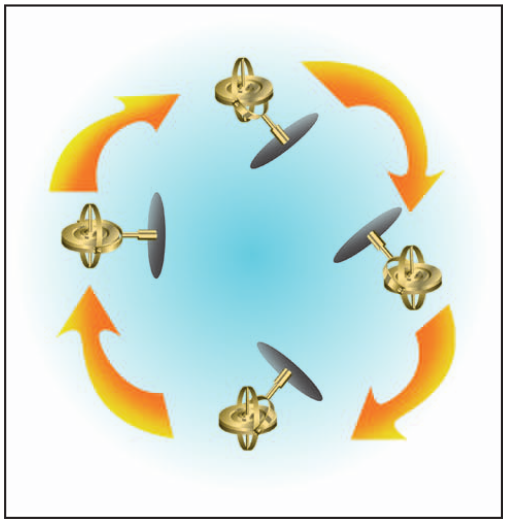
\includegraphics[scale=0.5]{figuras/giroscopo-rigidez.png}
	\captionof{figure}{\emph{Sin importar la posición de la base, el giróscopo mantiene su posición de rotación}.}
\label{fig:rigidez}
\end{center}

\subsubsection*{Precesión}
La precesión es el movimiento de giro de un giróscopo en respuesta a una fuerza de deflexión. La reacción de esta fuerza no ocurre en el punto donde fué aplicado, sino en un punto a 90º después de la dirección de rotación.

\begin{center}
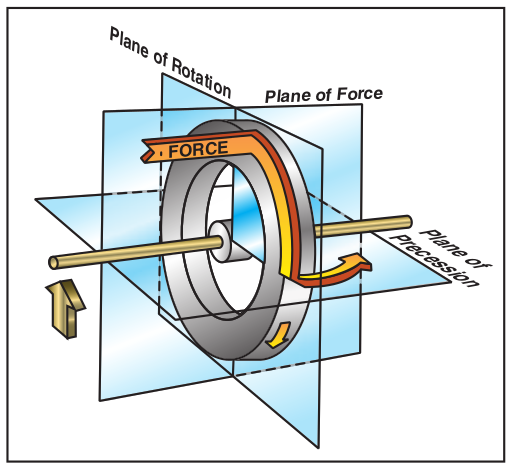
\includegraphics[scale=0.5]{figuras/giroscopo-precesion.png}
	\captionof{figure}{\emph{Preseción de un giróscopo como resultado de aplicar una fuerza de deflexión}.}
\label{fig:presecion}
\end{center}

\subsubsection*{Fuentes de poder}
En algunos aviones, todos los giros operan con vacio, presión o a electricidad; En otros, el indicador de dirección de actitud son a vacío o presión mientras que el coordinador de viraje es  alimentado electricamente. La mayoría de los aviones tienen al menos dos fuentes de poder para asegurar una fuente de información sobre el \textbf{ladeo} si una fuente de poder falla.

El sistema a presión o vacío hace rotar los giróscopos succionando o soplando una corriente de aire sobre las aletas del mismo. La cantidad de presión o vacío necesario para operar varía, pero está generalmente entre 4,5 a 5,5 in.Hg.

El problema que presenta el sistema a presión o vacío es que no funciona por encima de 10.000 metros o bajo temperaturas inferiores a -37 ºC. Para aeronaves que superen estos límites se requieren instrumentos alimentados por un sistema eléctrico.

\subsubsection{Instrumentos}
Los instrumentos giroscópicos aeronáuticos más comunes son:
\begin{itemize}
\item El indicador de actitud (horizonte artificial)
\item El indicador de rumbo.
\item Instrumentos de ritmo de giro:
  \begin{itemize}
    \item El indicador de virage e inclinación (\emph{turn and slip}, bola y bastón)
    \item El coordinador de viraje (\emph{turn coordinator}) 
  \end{itemize}
\end{itemize}

\subsubsection{Bastón y bola}
El bastón y bola es el instrumento básico de ritmo de giro, también conocido como \emph{indicador de viraje} o \emph{giro-viraje}. El instrumento fué uno de los primeros utilizados por los pilotos para controlar el aeroplano, sin tener referencias visuales.

\begin{center}
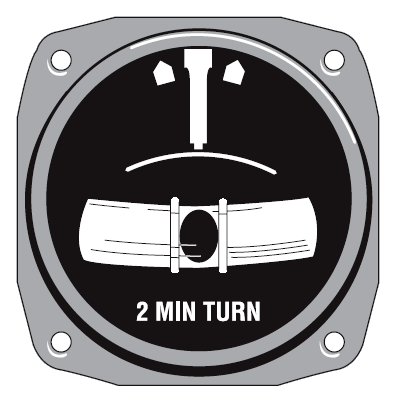
\includegraphics[scale=0.6]{figuras/Turn_and_slip}
	\captionof{figure}{\emph{Indicador de bastón y bola}.}
\label{fig:presecion}
\end{center}

En realidad, existen dos instrumentos en una sola carcasa; uno de ellos es el propio indicador de viraje (bastón)  y el otro es un inclinómetro.
El indicador de viraje es una aguja vertical bastante gruesa que puede oscilar hacia ambos lados. La parte giroscópica de este instumento doble es un volante de inercia que gira debido a un flujo de aire o por un motor eléctrico.

El rotor de indicador de viraje, formado por el volante de inercia, tiene el eje de giro paralelo al eje lateral del avión, y el eje del cardán es paralelo al eje longitudinal de la aeronave. Un resorte centrado sostiene el nivel del cardán cuando no existe ninguna fuerza exterior que actúe sobre él. Cuando el rotor está girando y el avión vira respecto a su eje vertical (eje de guiñada), actuá una fuerza sobre el eje del rotor a traveś del cardán, de forma que un lado del eje se mueve hacia delante y el otro lado hacia atrás.

La precesión origina la inclinación del rotor, como si la fuerza se sintiera noventa grados desplazada en el sentido de rotación del volante. Esta inclinación se contrarresta en algunos modelos con un resorte horizontal que se encla en un lado de la cuna, mientras que en otros modelos actúan dos fuerzas: una producida por un pistón que suaviza el esfuerzo y otra por un muelle calibrado que restringe la inclinación del cardán y se ancla en la parte inferor de la cuna.
\begin{center}
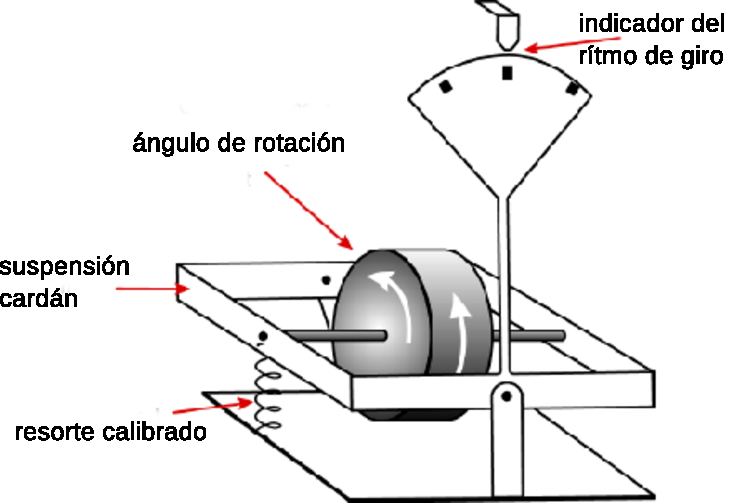
\includegraphics[scale=0.6]{figuras/turnandslip-spring.pdf}
	\captionof{figure}{\emph{Mecanismo del indicador de viraje}.}
\label{fig:presecion}
\end{center}

La aguja indica el movimiento del cardán, mostrando no sólo el ángulo de guiñada
sino también su ritmo.

La carcasa suele se una caja hermética que proteje al giróscopo del polvo y la humedad. Existen dos calibraciones estándar de este instrumento:

\begin{itemize}
  \item \textbf{Indicador de viraje de dos minutos}: El ritmo de giro estándar es de 3º por segundo, o lo que es lo mismo, se tarda dos minutos en dar una vuelta completa de 360º. En un viraje hacia la derecha, el borde izquierdo de la aguja se alinea con el borde derecho de la marca de índice.
  \item \textbf{Indicador de viraje de cuatro minutos}:  Con esta calibración  cuando la aguja se deflecta y se alinea con el indicador de izquierda o derecha, nos indica que estamos girando a un ritmo de giro de un grado y medio por segundo.
\end{itemize}

\subsubsection*{Inclinómetro}
El inclinómetro es un tubo curvado de cristal, relleno de un fluido amortiguador en cuyo interior se puede mover libremente una bola según la resultante de la fuerza centrífuga y gravitatoria. Para el piloto es un indicativo de uso de los alerones, en coordinación con el timón de dirección.

Cuando el ritmo de guiñada de una aeronave es correcto para un determinado ángulo de alabeo, observado en el indicador de viraje, la bola del inclinómetro se centrará entre las dos líneas que cruzan el tubo de cristal. 
La atracción de la graveda en la bola se ve afectada por la pendiente de tub: cuanto más empinado esté éste, mas tiene que esforzarse la bola para rodar hacia e extremo del tubo, cuyo sentido es el del ala mas baja. La fuerza centrífuga, por otro lado, empuja a la bola hacia la otra punta del tubo. Cuanto mayor es el ritmo de giro, mayor es la fuerza centrífuga, de forma que un viraje coordinado y equilibrado es aquel en e cual el ángulo de pendiente se corresponde con el ritmo de giro, por lo tanto la bola permanece centrada.

Para observar la calidad de un viraje, se diferencian los siguientes casos:

\begin{itemize}
  \item \textbf{Viraje coordinado}: Las fuerzas que actúan sobre la bola en todo momento son la gravedad y la fuerza centrífuga. Durante un viraje coordinado, ambas fuerzas permanecen en equilibrio, de forma que la bola no se mueve de su posición centrada en el interior del tubo. La bola continuará en su posición mientras no se desequlibren ambas fuerzas.

  \item \textbf{Derrape (skidding)}: Durante un derrape el ángulo de inlinación de la aeronave es muy pequeño respecto a la velocidad angular de viraje, por lo que la fuerza centrífuga desequilibra a la bola y hace que ésta se desplace hacia el extremo exterior del tubo durante el viraje.
  \item \textbf{Resbale o deslizamiento (slipping)}: En un resbala la velocidad angular del viraje es emasiado lenta para el ángulo de inclinaciión de la aeronave. El exceso de graveadd que actúa sobre la bola y lla falta de fuerza centrífuga provocan un deslizamiento de la bola en el interior del tubo hacia la parte interior del viraje. Ante este caso, el piloto debe disminuir el ángulo de alabeo o incrementar la velocidad angular de viraje (con más empuje).
\end{itemize}
 En síntesis, la bola se utiliza como un indicador de equilibrio en los virajes, ya que representa la relación existente entre las dos fuerzas principales que actúan durante el giro.

 \subsubsection*{Coordinador de viraje y alabeo (\emph{turn coordinator})}

 La evolución del instrumento \emph{bastón y bola} se denomina \textbf{coordinador de viraje y alabeo}. Un indicador de viraje sólo puede mostrar la rotación sobre el eje verticall del avión, es decir la guiñada. Como es sabido, un viraje aéro se comienza con un alabeo. Un indicador de viraje sería mucho mas valioso si también captase esta rotación.

 El mecanismo utilizado por un coordinador de viraje y alabeo es similar al de un indicador de viraje, excepto que el eje de su cardán está inclinado unos 30º, por lo que el giróscopo precesionará en caso de que el avión alabee o guiñe. Esto es especialmente deseable desde el punto de vista de que el indicador de viraje se ve afectado por el ángulo de guiñada adversa al principio del giro; sin embargo el coordinador de viraje capta el suficiente alabeo de las alas, que cancela cualquier deflexión causada por esta guiñada adversa.
 \begin{center}
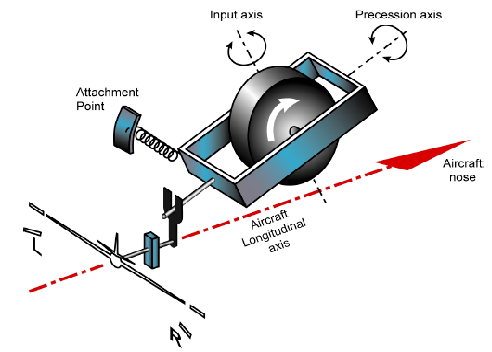
\includegraphics[scale=0.69]{figuras/Turn_coordinator-spring}
	\captionof{figure}{\emph{Mecanismo del coordinador de viraje}.}
\label{fig:tcspring}
\end{center}

\begin{center}
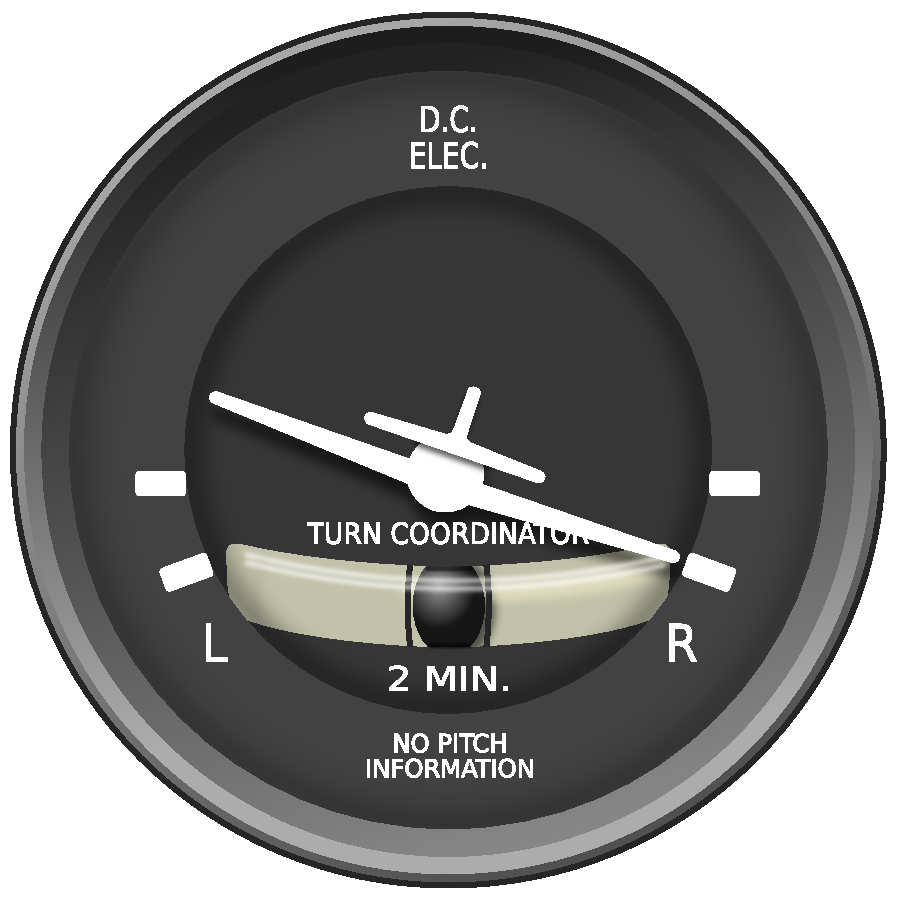
\includegraphics[scale=0.39]{figuras/Turn_coordinator}
	\captionof{figure}{\emph{Coordinador de viraje}.}
\label{fig:tc}
\end{center}

Este instrumento, utiliza el símbolo de un pequeño avión con marcas situadas en lo puntos opuestos del dial en los extremos de las alas. Cuando un avión gira a un ritmo normal hacia la izquierda, las alas del símbolo del avión se alinean con la marca del lado izquierdo del dial del instrumento, en concreto el marcado con $L$.


\subsubsection{Indicador de actitud}
El indicador de actitud se conoce comúnmente por horizonte artificial, pero también se conoce con varias denominaciones más: horizonte giroscópico, bola, giróscopo de actitud, instrumento de alabeo y cabeceo, indicador esférico...

El indicador de actitud proporciona al piloto la informacion de actitud de la aeronave respecto al horizonte terrestre real. Así, notifica el ángulo de alabeo y cabeceo comparados con el plano horizontal de la aeronave cuando se encuentre en vuelo recto y nivelado. Si un piloto está volando entre nubes, el piloto debe confiar en el horizonte artificial, y así determinar la actitud del avión y prevenir la pérdida de control. El horizonte artificial se convierte, de esta forma, en el instrumento más importante para el piloto en condiciones de vuelo por instrumentales (IFR).

\begin{center}
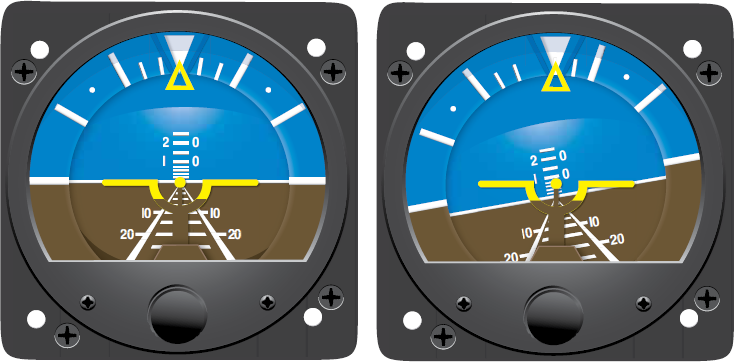
\includegraphics[scale=1.59]{figuras/horizonte-artificial}
	\captionof{figure}{\emph{Indicador de actitud}.}
\label{fig:AI}
\end{center}


\subsubsection*{Funcionamiento del indicador de actitud}
El indicacor de actitud opera apoyándose en la propiedad giroscópica de la rigidez espacial. Se compone de un giróscopo libre de rotación horizontal, con eje de giro vertical, montado sobre un sistema cardán que le confiere tres grados de libertad y que se mantiene en posición vertical gracias a un dispositivo sensible a la gravedad.

Cuando el avión realice algún cambio de actitud, es decir, alabee, encencabrite, pique o ejecute cualquier combinación de esos movimientos, la caja del instrumento realizará los mismos movimientos, por ir montados de forma fija en el avión; sin embaargo, el giróscopo interior del indicador mantendrá su plano de rotación debido a la propiedad de la rigidez espacial. Como la bola representativa de la Tierra persiste fija al giróscopo, el piloto puede visualizar los desplazamientos relativos y ser consciente en todo momento de la referencia del horizonte, pudiendo cuantificar con las escalas graduadas la actitud real de la aeronave. Este tipo de visualización no exige al piloto ningún esfuerzo adicional para la interpretación.
\begin{center}
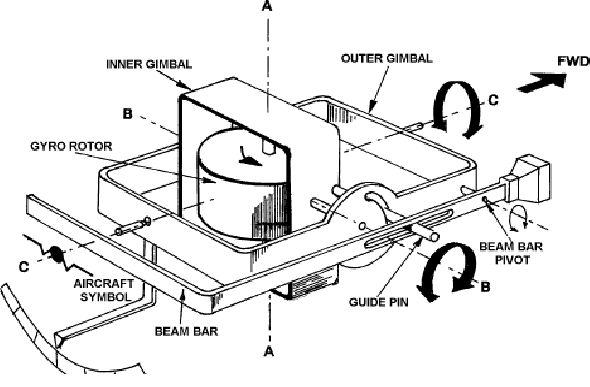
\includegraphics[scale=0.49]{figuras/horizonte-artificial-funcionamiento}
	\captionof{figure}{\emph{Funcionamiento del indicador de actitud}.}
\label{fig:FAI}
\end{center}


Es esencial reparar en que el horizonte artificial no proporciona al piloto información de si la aeronave asciende o desciende, ya que un centrado desplazado de la aeronave puede hacer que la proa suba o baje, independientemente de que el vector velocidad del avión sea horizontal. En estos casos, el piloto puede ajustar en el instrumento la altura del avioncito respecto a la línea del horizonte.

En las siguientes figuras se puede observar la interpretación de forma visual de distintas actitudes de la aeronave.

\begin{center}
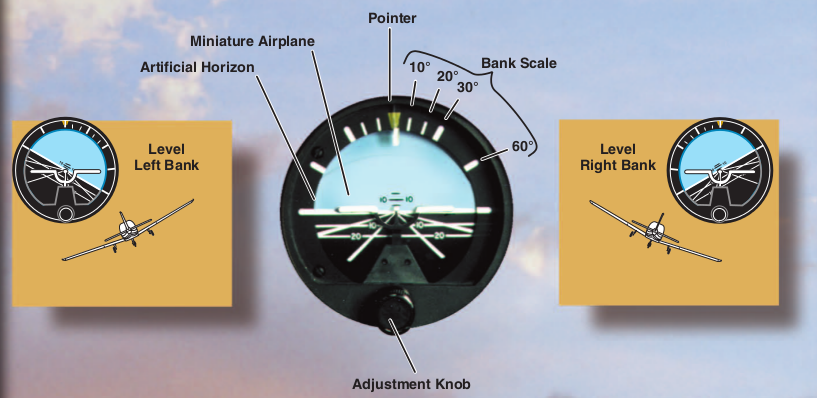
\includegraphics[scale=0.39]{figuras/ha}
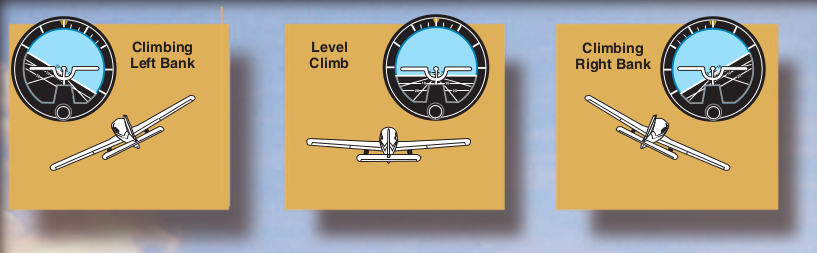
\includegraphics[scale=0.39]{figuras/ha-1}
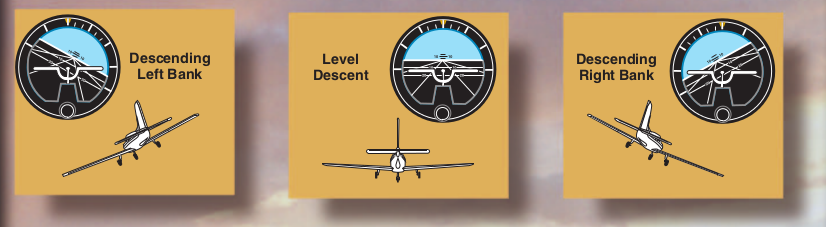
\includegraphics[scale=0.39]{figuras/ha-2}

\end{center}


\subsubsection*{Erección del indicador de actitud}
Antes de empezar a usar el indicador de actitud, el rotor debe estar girando en posición vertical (erecto). Para lograrlo se pueden utilizar sistemas eléctromecánicos o mecánicos que automáticamente posicionen el rotor al encender el equipo. 
\begin{center}
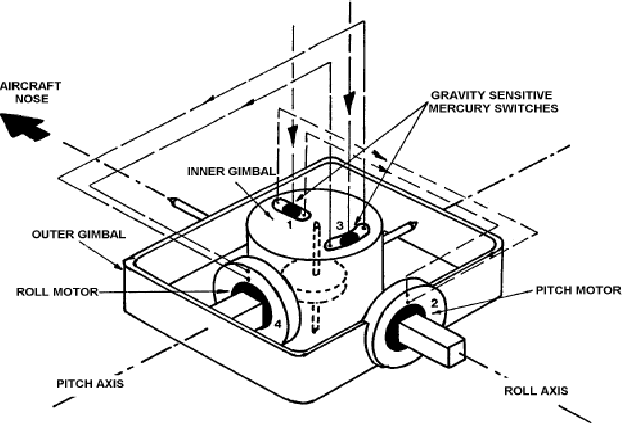
\includegraphics[scale=1.99]{figuras/horizonte-artificial-funcionamiento-2}
\captionof{figure}{\emph{Sistema de erección con motores eléctricos}.}
\label{fig:SAI}
\end{center}


\end{document}

